\section{V4}

\subsection{Cortex-M3/M4}
\begin{multicols}{2}

\begin{itemize}
    \item Harvard Architecture
    \subitem \rightarrow Zugriffe auf Instruktionen und Daten \newline
    können gleichzeitig stattfinden
    \item Internal Bus Interconnect
    \subitem \rightarrow mehrere Bus-Interface 
    \item Nested Interrupt Controller \textbf{(NVIC)}
    \item Standart Timer \textbf{(SYSTICK)}\\
    \textbf{Optional:}
    \item Memory Protection Unit \textbf{(MPU)}
    \item Floating Point Unit \textbf{(FPU)}
\end{itemize}

\end{multicols}
\subsection{System-Komponenten}
\begin{multicols}{2}
\begin{minipage}{\linewidth}
    \subsubsection{NVIC}
    \begin{itemize}
    \item Non-Maskable Interrupt (NMI)
    \item Bis zu 240 externe Interrupts
    \item 8 bis 256 Prioritätslevel
    \end{itemize}
    \rightarrow ISR benötigt 12 Taktzyklen\\
\end{minipage}
\begin{minipage}{\linewidth}
    \subsubsection{FPU - (nur Cortex M4!)}
    Mit der FPU lassen sich IEEE754 Signal Precision Floating-Point Operationen in sehr wenigen Takten ausführen\\
\end{minipage}
\begin{minipage}{\linewidth}
    \subsubsection{WIC (Wakeup Interrupt Controller)}
    Für die Umsetzung von Low-Power-Modes\newline
    Dadruch kann 99\% der Cortex M3-Prozessoren im Low-Power-Bereich arbeiten.
    \newline
    Ist mit dem NVIC verknüpft und holt den Prozessor aus diesem Modus heraus, um auf einen Interrupt reagieren zu können\\
\end{minipage}
\begin{minipage}{\linewidth}
    \subsubsection{SYSTICK}
    \begin{itemize}
    \item 24-Bit Countdown-Timer mit automatischer Relaod-Funktion
    \item Wird für einen periodischen Interrupt verwendet
    \end{itemize}
    Wenn der Zähler den Wert 0x000000, wird dies dem NVIC signalisiert und  der Reload-Wert wird aus dem Reload-Register gelesen.
    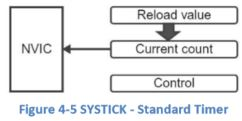
\includegraphics[width=6cm]{images/NVIC}\\
\end{minipage}
\begin{minipage}{\linewidth}
    \subsubsection{MPU}
    \begin{itemize}
    \item ermöglicht Zugriffsregel für den Privilieged Access und User Programm Access zu definieren
    \item \rightarrow Wird eine Zugriffsrege verletzt erfolgt eine Exception-Regelung wodurch der Exceptrion Handler das Problem analysiert und ggf. beheben kann
    \item \rightarrow Ausserdem ist es möglich gewisse Bereiche als read-only zu deklarieren
    \end{itemize}
\end{minipage}
\end{multicols}
\clearpage

\subsection{GNU-Tool-Chain Entwicklungsablauf}
\begin{multicols}{2}
          \begin{minipage}{\linewidth}
    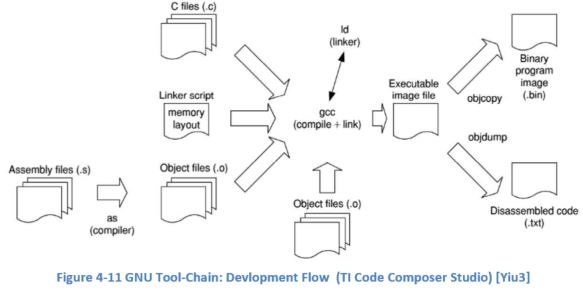
\includegraphics[width=\textwidth]{images/gnutoolchain}
    \begin{tabular}{|l|l|}
        \hline 
        \textbf{APSR}& Application Program Status Register \\ 
        \hline 
        \textbf{IPSR}& Interrupt Program Status Register \\ 
        \hline 
        \textbf{EPSR}& Execution Program Status Register \\ 
        \hline 
    \end{tabular}
    \subsubsection{SP-zugriffe(Assembler)}
      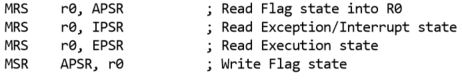
\includegraphics[width=\textwidth]{images/SPzugriffe}   
\end{minipage}
    
    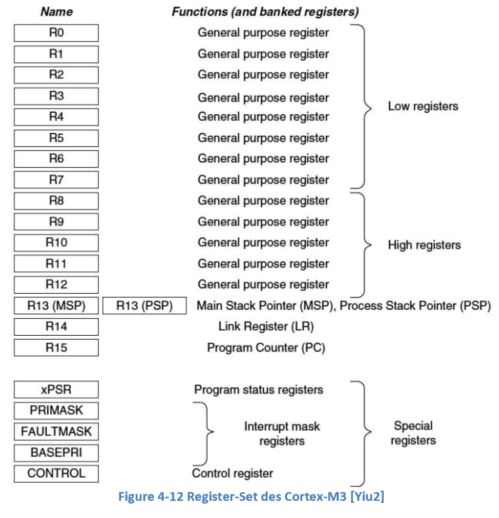
\includegraphics[width=0.5\textwidth]{images/gnutoolchain1}
\end{multicols}

\subsection{Programm Status Register}
\begin{minipage}{\linewidth}
    \begin{tabular}{|l|l|}
        \hline 
        \textbf{N}& Negativ \\ 
        \hline 
        \textbf{Z}& Zero  \\ 
        \hline 
        \textbf{C}& Carry/borrow  \\ 
        \hline 
        \textbf{V}& Overflow \\ 
        \hline 
        \textbf{Q}& Sticky saturation flag \\ 
        \hline 
        \textbf{ICI/IT}& Interrupt-Continauble Instruction(ICE) bits\\
                        & IF-THEN instruction status bit \\ 
        \hline 
        \textbf{T}& Thumb state, always 1; Trying to clear this bit will caus a fault exception \\ 
        \hline 
        \textbf{Exception number}& INdicates whiche exception the processor is handeling \\ 
        \hline 
    \end{tabular} 
\end{minipage}

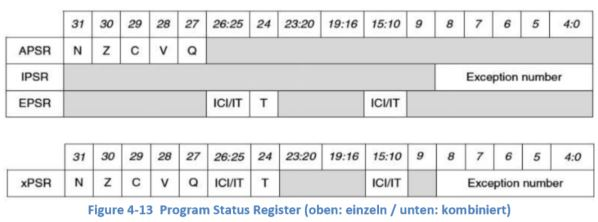
\includegraphics[width=17cm]{images/programstatusregister}
\clearpage

\subsection{Stack}
\begin{multicols}{2}
\begin{minipage}{0.5\textwidth}
    \begin{itemize}
        \item Temporäre Zwischenspeicherung von Daten während der ausführung einer Funktion
        \item Übergabe von Informationen an Funktionen oder Subroutinen
        \item Speichern von lokalen Variabeln
        \item Erhalten von Prozessor-Status und Register-Werten, während Exceptions oder Interrupts ausgefüht werden
        \item PUSH-POP-Instruktionen werden ausgeführt
        \item LIFO-Prinzip(Last In, First Out)
    \end{itemize}
\end{minipage}

\begin{minipage}{0.5\textwidth}
    \subsubsection{Main-Stak-Pointer (MSP)}
    \begin{itemize}
        \item Standart Stack Pointer nach einem Reset
        \item Innerhalb von Exception-INterrupt-Handler wird imer der MSP benutzt!
        \end{itemize}
    \subsubsection{Prozesor-Stack-Pointer (PSP)}
    \begin{itemize}
        \item Alternativer Stackpointer
        \item Wird nur im Thread-Mode verwendet
        \subitem \rightarrow bei embedded OS-System
    \end{itemize}   
\end{minipage}
\end{multicols}

















